
\section{Conceitos}
\label{section:redes:conceitos}

Newman \cite{newman:2018:networks} define uma rede da seguinte forma: \aspas{Uma \textbf{rede} é, em sua forma mais simples, uma coleção de pontos unidos em pares por linhas. Na nomenclatura da área um ponto é chamado \textbf{nó} ou \textbf{vértice} e a linha é chamada \textbf{aresta}}.  Uma rede é também chamada de \textbf{grafo} na literatura matemática.

A quantidade de vértices de um grafo $G$ é denotado por $n$ e a quantidade de arestas é denotado por $m$. Uma aresta que conecta um vértice a ele mesmo é chamado \textbf{ciclo}. Um grafo pode ter mais de uma aresta entre dois vértices, neste caso estas são chamadas \textbf{multiarestas}, e o grafo é chamado \textbf{multigrafo}. Um grafo que não possui ciclos é chamado \textbf{grafo acíclico}. Um grafo que não possui ciclos nem multiarestas é chamado \textbf{grafo simples}.

As arestas de um grafo podem ou não possuir uma direção associada, indicando que cada aresta parte de um vértice em direção a outro. Um grafo que possui arestas direcionadas é chamado \textbf{grafo direcionado}, também chamado \textbf{dígrafo}, caso contrário é chamado \textbf{grafo não-direcionado}. As arestas de um grafo também podem ou não possuir valores associados, chamados de \textbf{pesos}. Um grafo que possui pesos é chamado \textbf{grafo ponderado}.

\section{Representação}
\label{section:redes:representacao}

Um grafo é comumente representado por uma matriz de adjacências na forma:

\begin{equation}
A_{ij} = \begin{cases}
1 & \mbox{se existe uma aresta entre os vértices i e j,}\\
0 & \mbox{caso contrário}
\end{cases}
\end{equation}

No caso de um grafo ponderado, a matriz toma a seguinte forma:

\begin{equation}
A_{ij} = \begin{cases}
w_{ij} & \mbox{se existe uma aresta entre os vértices i e j de peso $w_{ij}$,}\\
0 & \mbox{caso contrário}
\end{cases}
\end{equation}

\begin{figure}[htb]
 \caption{Exemplo de grafo acíclico direcionado não-ponderado}
 \label{fig:redes1:grafo-exemplo}
 \centering
 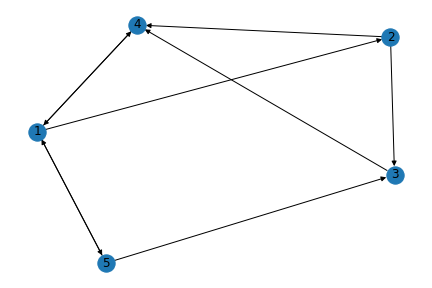
\includegraphics[scale=0.7]{images/redes-1-grafo-exemplo.png}
 \fautor
\end{figure}

A figura \ref{fig:redes1:grafo-exemplo} representa um grafo que pode ser representado pela matriz:

\begin{equation}
A = \begin{bmatrix}
0 & 1 & 0 & 1 & 1 \\
0 & 0 & 1 & 1 & 0 \\
0 & 0 & 0 & 1 & 0 \\
1 & 0 & 0 & 0 & 0 \\
1 & 0 & 1 & 0 & 0 \\
\end{bmatrix}
\end{equation}

outros conceitos usados na seção seguinte

\section{Métricas}
\label{section:redes:metricas}

descricao das métricas usadas
